%\documentclass[11pt,letterpaper]{article}
\documentclass[14pt,letterpaper]{extarticle}

% ----------------------------------
%            PAQUETES
% ----------------------------------
\usepackage[spanish]{babel}
\usepackage[utf8]{inputenc}
\usepackage[T1]{fontenc}
\usepackage{lmodern}  
\usepackage{csquotes}
\usepackage{setspace}           % Interlineado
\usepackage{geometry}           % Márgenes

							          % Hipervínculos
\usepackage{titlesec}           % Formato de títulos
\usepackage{tocloft}            % Formato de tabla de contenido
\usepackage{filecontents}
\usepackage{graphicx}
\usepackage{apacite}            % Estilo APA
\usepackage{indentfirst}        % Sangría en primer párrafo


\onehalfspacing                 % Interlineado 1.5
\graphicspath{{./Imagenes/}}
\usepackage{float}
\restylefloat{figure}
\usepackage{amsmath}



% ----------------------------------
%            FORMATO APA
% ----------------------------------
\geometry{left=2.54cm, right=2.54cm, top=2.54cm, bottom=2.54cm}
\onehalfspacing     % Interlineado 1.5

% Estilo de títulos APA
\titleformat{\section}{\normalfont\bfseries\large}{\thesection.}{0.5em}{}
\titleformat{\subsection}{\normalfont\bfseries\normalsize}{\thesubsection.}{0.5em}{}

% ----------------------------------
%        PORTADA TIPO APA
% ----------------------------------
\title{\textbf{Título del Informe}}
\author{Marlon Iván Carreto Rivera}
\date{\today}


\usepackage{pdfpages}
\usepackage{hyperref} 
\hypersetup{
	colorlinks=true,
	linkcolor=black,
	urlcolor=black,
	citecolor=black
}









% ----------------------------------
\begin{document}
	
		
\includepdf[pages=-,pagecommand={}]{Caratula/Caratulaanteproyecto.pdf}
	%%
\includepdf{Caratula/Caratulaanteproyecto.pdf}
	%\maketitle
	\thispagestyle{empty}


	\newpage
	
	
	
	
	
	
	% ----------------------------------
	%      TABLA DE CONTENIDO
	% ----------------------------------
	\renewcommand{\contentsname}{Contenido}
	\tableofcontents
	\newpage
	

	
	% ----------------------------------
	%        CONTENIDO DEL INFORME
	% ----------------------------------
	
	\section*{Introducción }
	
	% --- Introducción (sin numerar, con link funcional) ---
	\phantomsection
	El diseño estructural sismorresistente constituye uno de los aspectos fundamentales en la ingeniería civil, especialmente en regiones expuestas a amenazas sísmicas significativas. Dentro de los diferentes sistemas estructurales utilizados en edificaciones, los pórticos resistentes a momento destacan por su capacidad para resistir cargas verticales y horizontales, así como por su comportamiento dúctil frente a acciones sísmicas. Estos sistemas permiten una adecuada disipación de energía, control de desplazamientos y una mayor flexibilidad arquitectónica, factores clave para garantizar la seguridad estructural y funcional de las edificaciones. 	\\
	El presente trabajo aborda de manera integral los principales tipos de sistemas estructurales de pórticos, haciendo énfasis en los pórticos especiales, intermedios y ordinarios a momento, así como en los criterios normativos que rigen su diseño. Se analiza el comportamiento estructural de estos sistemas, considerando aspectos como la distribución de momentos, el control de desplazamientos, la capacidad de disipación de energía y el diseño por capacidad, elementos esenciales para un desempeño sísmico adecuado.
	
		\newpage
	% ----------------------------------
	\section{Tipos de Sistemas Estructurales}


	
	La clasificación tipológica de las estructuras es clave en la ingeniería sísmica en Guatemala, ya que define la forma en que los edificios resisten y transmiten tanto las cargas gravitacionales como las fuerzas laterales (sismos y viento) hacia la cimentación. Para lograr una adecuada comprensión de estos sistemas, las normas de diseño estructural AGIES los agrupan oficialmente en las siguientes categorías principales:
	
	\subsection{Sistema E1, Estructua de Marcos Simples }
	
	
	
	Es un sistema estructural tridimensional constituido únicamente por un conjunto de columnas y vigas. Su rasgo principal es que estos marcos, conectados de forma rígida, soportan la totalidad de las cargas verticales y también resisten completamente las acciones horizontales (como sismos y viento) mediante esfuerzos de flexión y corte. Además, todos los marcos deben estar interconectados mediante diafragmas de piso rígidos.
	

	Aquí lo tienes comenzando desde una **subsubsection** y con la redacción modificada:
	
	```latex
	\subsubsection{Materiales, Ductilidad y Parámetros de Diseño}
	
	Las estructuras pueden ejecutarse empleando concreto reforzado (conforme a NSE 7.1), perfiles de acero estructural (NSE 7.5) o sistemas mixtos de acero–concreto. De acuerdo con la rigidez de las conexiones en los nudos y el nivel de confinamiento que presentan, se clasifican en tres categorías: Alta Ductilidad (DA), Ductilidad Intermedia (DI) y Baja Ductilidad (DB).
	
	Con base en lo establecido en la normativa (Ref.: NSE 3, Tabla 6.1.4-1 y Tabla 4.3.3), se definen los siguientes parámetros de diseño:
	
	\begin{itemize}
		\item \textbf{Alta Ductilidad (DA):} Posee un factor de reducción $R = 8$, un factor de sobrerresistencia $\Omega = 3$ y un factor de amplificación de desplazamientos $C_d = 5.5$. No presenta restricciones de altura en ninguna zona sísmica.
		
		\item \textbf{Ductilidad Intermedia (DI) en concreto:} Considera $R = 5$, $\Omega = 3$ y $C_d = 4.5$. No se permite (NP) su uso en zonas de alta amenaza sísmica, correspondientes a las zonas D y E.
		
		\item \textbf{Baja Ductilidad (DB) en concreto:} Presenta valores de $R = 3$, $\Omega = 3$ y $C_d = 2.5$. Se limita a una altura máxima de 20 metros y no se permite en las zonas sísmicas C, D y E.
	\end{itemize}
	
	
		\begin{figure}[H]
		\centering
		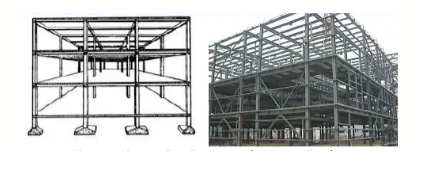
\includegraphics[width=0.8\textwidth]{E1}
		
		\label{fig:mi_imagen}
	\end{figure}



	
	\subsection{Sistema E2, Estructura de muros o Estructura tipo cajón}
	
	El sistema estructural de muros, también conocido como sistema tipo cajón, se caracteriza por estar conformado por elementos verticales continuos que trabajan de manera conjunta, interconectados mediante losas que actúan como diafragmas rígidos. Estas losas permiten la adecuada distribución de las cargas hacia los muros estructurales, garantizando un comportamiento integral del sistema tridimensional.
	
	En este tipo de estructuras, los muros son los principales responsables de resistir la totalidad de las acciones laterales, tales como las fuerzas sísmicas y de viento, así como una proporción significativa o la totalidad de las cargas gravitacionales. Cuando se incorporan columnas aisladas, estas cumplen principalmente la función de soportar cargas verticales, pero no participan de manera significativa en la resistencia ante solicitaciones sísmicas.
	

	
	\subsubsection{Materiales y ductilidad}
	
	Los sistemas de muros estructurales se construyen principalmente utilizando concreto reforzado o mampostería reforzada, ya sea tradicional o confinada. En el caso del concreto, el nivel de ductilidad puede clasificarse como Alta Ductilidad (DA) o Ductilidad Baja (DB), dependiendo de los requisitos de detallado y confinamiento establecidos en la normativa correspondiente. 
	

	
	La ductilidad del sistema es un aspecto fundamental en zonas sísmicas, ya que permite disipar energía mediante deformaciones inelásticas controladas, reduciendo el riesgo de fallas frágiles.
	
	\subsubsection{Parámetros de diseño (ref.: nse 3, tabla 6.1.4-1 y nse 7.9, tabla 4.4-1)}
	
	De acuerdo con las disposiciones normativas, los parámetros de diseño para los sistemas de muros se definen en función de su capacidad resistente y ductilidad, considerando factores que modifican las fuerzas sísmicas de diseño:
	
	\begin{itemize}
		\item \textbf{Concreto de Alta Ductilidad (DA):} Se adoptan valores de $R = 6$, $\Omega = 2.5$ y $C_d = 5$. La deriva máxima permisible es de 2\% (0.020$h$), lo que indica una buena capacidad de deformación bajo cargas sísmicas.
		
		\item \textbf{Concreto de Baja Ductilidad (DB):} Se consideran $R = 4$, $\Omega = 2.5$ y $C_d = 4$. La deriva máxima permitida se restringe a 1\% (0.010$h$), reflejando una menor capacidad de disipación de energía.
		
		\item \textbf{Mampostería Reforzada (DA):} Presenta valores típicos de $R = 4$, $\Omega = 2.5$ y $C_d = 3.5$, siendo un sistema con comportamiento intermedio en términos de rigidez y ductilidad.
		
		\item \textbf{Mampostería de pequeña vivienda (DB):} Utiliza $R = 3$, $\Omega = 2.5$ y $C_d = 2$, adecuado para edificaciones de baja altura con limitadas demandas sísmicas.
	\end{itemize}
	
	Los sistemas clasificados como de baja ductilidad presentan penalizaciones en el diseño debido a su limitada capacidad de disipar energía, lo que implica mayores fuerzas de diseño y menores deformaciones permisibles. Esto se debe a que estos sistemas son más susceptibles a fallas frágiles, especialmente por aplastamiento o agrietamiento en compresión.
	



		\begin{figure}[H]
		\centering
		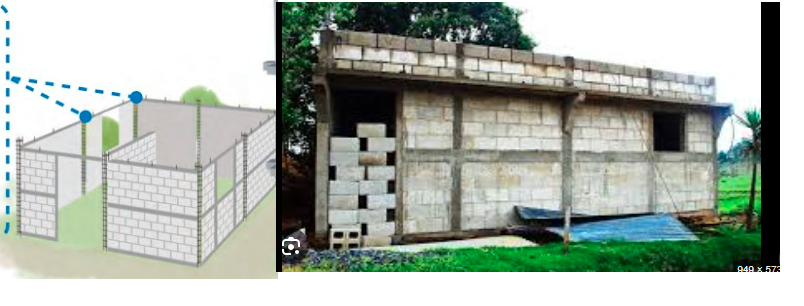
\includegraphics[width=1\textwidth]{E2}
		
		\label{fig:mi_imagen}
	\end{figure}
	


	\subsection{Sistema E3, Estructura Combinada}
	
	El sistema estructural combinado corresponde a una configuración en la que se integran muros estructurales con marcos resistentes, los cuales pueden incluir marcos simples o marcos arriostrados mediante diagonales. En este tipo de sistema, las cargas laterales, como las provenientes de sismos o viento, se distribuyen entre los muros y los marcos en función de su rigidez relativa, lo que permite un comportamiento estructural más eficiente y equilibrado.
	

	
	Adicionalmente, estudios técnicos y tesis en ingeniería estructural señalan que este tipo de sistema mejora la redundancia estructural y proporciona rutas alternas para la disipación de energía, lo cual resulta favorable ante eventos sísmicos severos.
	
	\subsubsection{Materiales y ductilidad}
	
	Los sistemas combinados pueden construirse utilizando muros de concreto reforzado clasificados como de Alta Ductilidad (DA) o Baja Ductilidad (DB), así como mampostería reforzada en categoría de Alta Ductilidad (DA). Estos muros se integran con marcos de concreto o acero estructural.
	

	
	
	\subsubsection{Parámetros de diseño (ref.: nse 3, tabla 6.1.4-1)}
	
	De acuerdo con la normativa aplicable, los parámetros de diseño para este tipo de sistema dependen del grado de ductilidad y del tipo de elementos estructurales que lo conforman:
	
	\begin{itemize}
		\item \textbf{Concreto de Alta Ductilidad (DA) (muros y marcos):} Se consideran valores de $R = 6$, $\Omega = 2.5$ y $C_d = 5$. Este sistema no presenta limitaciones de altura, debido a su adecuado comportamiento sísmico.
		
		\item \textbf{Acero con riostras excéntricas (DA):} Se adoptan valores de $R = 8$, $\Omega = 2.5$ y $C_d = 4$. Este sistema tampoco presenta restricción en altura, ya que ofrece una alta capacidad de disipación de energía mediante deformaciones inelásticas controladas.
		
		\item \textbf{Acero con riostras concéntricas (DB):} Presenta valores de $R = 3.25$, $\Omega = 2$ y $C_d = 3.25$. En este caso, la altura de la edificación se limita generalmente en un rango de 12 a 20 metros, debido a su menor capacidad de disipación de energía.
	\end{itemize}
	
	\subsubsection{Comportamiento estructural}
	
	En este tipo de sistema, la distribución de fuerzas laterales depende directamente de la rigidez relativa entre los muros y los marcos. En general, los muros estructurales tienden a absorber la mayor parte del cortante basal debido a su mayor rigidez, mientras que los marcos contribuyen principalmente en el control de deformaciones y en la redistribución de esfuerzos.
	
	\begin{figure}[H]
		\centering
		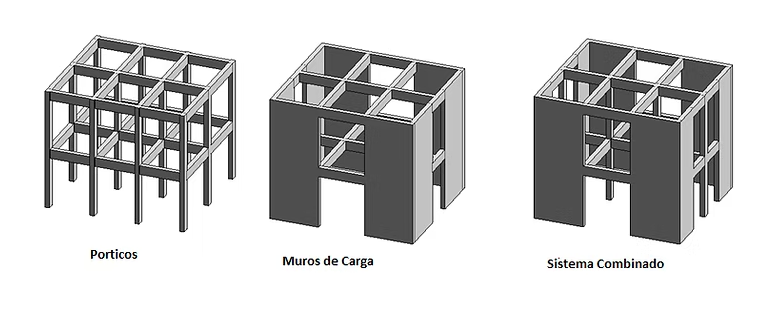
\includegraphics[width=1\textwidth]{E3}
		
		\label{fig:mi_imagen}
	\end{figure}
	

	\subsection{Sistema E4, Estructura Dual}
	
	Este sistema es visualmente similar al Sistema E3; sin embargo, cuenta con un refuerzo normativo basado en una “doble línea de defensa”. Para que una estructura sea considerada dual, debe cumplir dos condiciones estrictas: 
	
	\begin{itemize}
	\item Los muros estructurales deben resistir al menos el 40\% de las fuerzas sísmicas de cada nivel.
	\item Los marcos de vigas y columnas, los cuales deben ser obligatoriamente de Alta Ductilidad, se diseñan para resistir de manera independiente al menos el 25\% del sismo total, considerando la posible falla de los muros.
	\end{itemize}

	
	\subsubsection{materiales y ductilidad}
	
	Se emplean marcos de concreto de Alta Ductilidad (DA) combinados con muros de concreto también de Alta Ductilidad. Asimismo, pueden utilizarse marcos de acero de Alta Ductilidad con riostras, ya sean excéntricas o concéntricas, igualmente diseñadas bajo criterios de ductilidad elevada.
	
	\subsubsection{parámetros de diseño (ref.: nse 3, tabla 1.6.14-1)}
	
	\begin{itemize}
		\item \textbf{Concreto DA (marcos y muros):} $R = 7$, $\Omega = 2.5$, $C_d = 5.5$. No presenta límite de altura.
		
		\item \textbf{Acero DA con riostras excéntricas:} $R = 8$, $\Omega = 2.5$, $C_d = 4$. Sin límite de altura.
	\end{itemize}
	
	\subsubsection{desempeño del sistema}
	
	Este sistema es uno de los más favorecidos para edificaciones de gran altura, ya que la condición de que los marcos dúctiles resistan al menos el 25\% del sismo de manera independiente permite evitar el colapso gravitacional, incluso ante una posible falla severa de los muros estructurales.


		\begin{figure}[H]
		\centering
		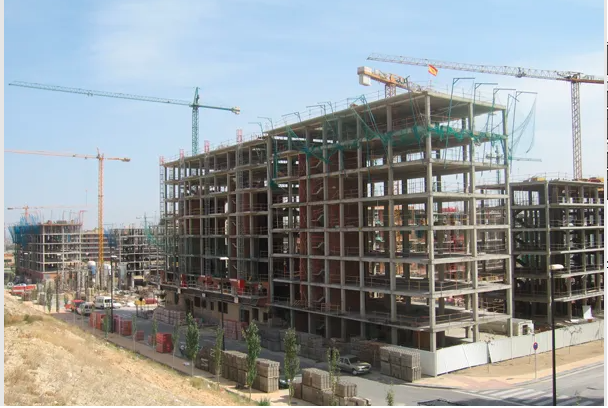
\includegraphics[width=0.6\textwidth]{E4}
		
		\label{fig:mi_imagen}
	\end{figure}




	\subsection{Sistema E5, Soportes en Voladizo y Naves}
	
	Son estructuras generalmente de un solo nivel, como naves industriales, bodegas, pabellones o remates superiores, en las cuales las columnas o muros trabajan como elementos en voladizo empotrados en su base, soportando la totalidad de la carga horizontal sin la participación de un marco superior en esa dirección.
	
	\subsubsection{Materiales y ductilidad}
	
	Se emplean columnas de concreto reforzado con confinamiento, perfiles de acero con detallado sísmico, así como naves construidas en mampostería o columnas de madera.
	
	\subsubsection{Parámetros de diseño (ref.: nse 3, tabla 1.6.14-1)}
	
	\begin{itemize}
		\item \textbf{Concreto confinado / acero sísmico:} $R = 2.5$, $\Omega = 1.25$, $C_d = 2.5$. Límite de altura de 12 metros.
		
		\item \textbf{Naves de mampostería:} $R = 2$, $\Omega = 1.25$, $C_d = 2$. Límite de altura de 6 metros.
	\end{itemize}
	
	\subsubsection{Consideraciones estructurales}
	
	Debido a la ausencia de múltiples ejes y redundancia, la demanda axial en la columna bajo carga sísmica no debe superar el 25\% de su capacidad. Además, el diseño del momento flector en la cimentación y en la base de la columna se incrementa obligatoriamente mediante el factor de sobrerresistencia $\Omega$.


		\begin{figure}[H]
		\centering
		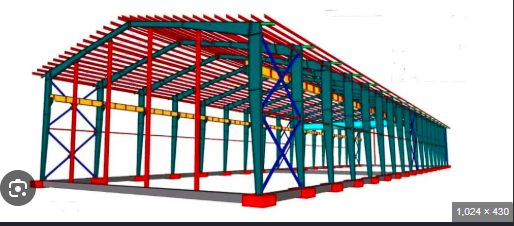
\includegraphics[width=0.8\textwidth]{E5}
		
		\label{fig:mi_imagen}
	\end{figure}
	
	
	
	\subsection{Sistema E6, Péndulo Invertido}
	
	Se trata de un soporte central o de un conjunto de soportes aislados que funciona como un voladizo vertical, en donde más del 50\% de la masa se concentra en la parte superior, como ocurre en los tanques elevados de agua. La estabilidad lateral depende completamente de la restricción a momento en la base.
	
	\subsubsection{Materiales y Ductilidad}
	
	Se utilizan materiales como concreto confinado o acero con detallado sísmico rígido.
	
	\subsubsection{Parámetros de diseño (ref.: nse 3, tabla 1.6.14-1)}
	
	En sistemas de concreto y acero, se aplica el mayor nivel de exigencia normativa debido a su condición de inestabilidad. Se consideran los siguientes valores: $R = 2$, $\Omega = 1.5$, $C_d = 1.5$. Se establece un límite de altura de 15 metros en zonas de alta sismicidad (Nivel E).
	
	\subsubsection{Consideraciones estructurales}
	
	La demanda de carga axial en la columna principal se limita de forma estricta, ya que no debe sobrepasar el 15\% de la resistencia axial concéntrica del elemento. Esto asegura que el concreto no falle por compresión durante la acción de flexión inducida por el sismo.
	
	












	

	\subsection{comportamiento de los sistemas estructurales}
	
	El comportamiento de los sistemas estructurales, bajo la normativa técnica guatemalteca, se fundamenta en la capacidad de la edificación para gestionar la energía sísmica y mantener la estabilidad bajo distintas intensidades de carga. Este comportamiento se analiza a través de los siguientes niveles y principios mecánicos:
	
	\subsubsection{1. Rangos de Desempeño Mecánico}
	
	El comportamiento de cualquier sistema estructural se divide estrictamente según la magnitud de la fuerza aplicada:
	
	\begin{itemize}
		\item \textbf{Rango Elástico (Solicitaciones Frecuentes):} Ante cargas gravitacionales permanentes, viento o sismos de baja intensidad, la estructura debe comportarse de forma elástica, absorbiendo la carga sin experimentar deterioro estructural ni deformaciones permanentes.
		
		\item \textbf{Rango Post-Elástico (Sismos Severos):} Para eventos sísmicos máximos de diseño, se permite intencionalmente que los componentes incursionen en el rango post-elástico. En este estado, se admite la posibilidad de daño (incluso no reparable) con el objetivo primario de disipar energía mediante una \textbf{cedencia controlada} para salvar vidas.
	\end{itemize}
	
	\subsubsection{2. Principios de Integridad y Continuidad}
	
	Para que el comportamiento sea global y no falle de forma aislada, se deben cumplir dos principios:
	
	\begin{itemize}
		\item \textbf{Trayectoria de Cargas:} Debe existir una o varias rutas continuas que transmitan las fuerzas inerciales desde el punto de origen hasta la cimentación. Si esta ruta se interrumpe (como en muros discontinuos), es obligatorio aplicar factores de sobre-resistencia ($\Omega_r$) para evaluar la transferencia local.
		
		\item \textbf{Integridad Estructural:} Todos los elementos deben estar interconectados mediante conexiones diseñadas formalmente, incluyendo el anclaje de losas a muros y de la estructura a sus apoyos.
	\end{itemize}
	
	\subsubsection{3. Acción Dinámica del Diafragma}
	
	Las losas de entrepiso y techo (diafragmas) actúan como colectores y distribuidores de fuerzas:
	
	\begin{itemize}
		\item \textbf{Distribución por Rigidez:} En diafragmas rígidos, la fuerza sísmica se reparte entre los miembros verticales (columnas o muros) según su rigidez relativa.
		
		\item \textbf{Efectos de Torsión:} Se debe considerar el momento de giro provocado por la excentricidad entre el centro de masa y el centro de rigidez, sumando una \textbf{excentricidad accidental adicional del 5\%}.
		
		\item \textbf{Diafragmas Flexibles:} En techos ligeros (como lámina) sin rigidez cortante, las fuerzas se aplican independientemente a cada elemento según su área tributaria.
	\end{itemize}
	
	\subsubsection{4. Inestabilidad y Efectos de Segundo Orden (P-Delta)}
	
	El comportamiento lateral se ve agravado por los efectos \textbf{P-Delta}. Cuando el edificio sufre desplazamientos laterales ($\Delta$), las masivas cargas gravitacionales ($P$) se desalinean de sus ejes de soporte, generando un momento de volteo adicional que empuja a la estructura a inclinarse más, pudiendo causar colapso gravitacional post-sismo si no se corrige en el diseño.
	
	\subsubsection{5. Niveles de Desempeño y Daño Esperado}
	
	La normativa parametriza el comportamiento físico esperado en tres niveles:
	
	\begin{itemize}
		\item \textbf{Operacional (OP):} Los componentes estructurales y no estructurales mantienen sus funciones; obligatorio para hospitales y obras esenciales.
		
		\item \textbf{Seguridad de la Vida (SV):} Se admite daño estructural significativo y agrietamientos, pero se mantiene un margen de seguridad claro contra el derrumbe para permitir la evacuación.
		
		\item \textbf{Prevención del Colapso (PC):} Límite extremo donde hay distorsiones excesivas y ruina irrecuperable, pero la estructura sigue sosteniendo las cargas verticales para evitar fatalidades.
	\end{itemize}
	
	\subsubsection{6. Comportamiento según el Sistema Tipológico (E1 a E7)}
	
	Cada sistema tiene un mecanismo de resistencia único que dicta su respuesta:
	
	\begin{itemize}
		\item \textbf{Marcos (E1):} Resisten mediante flexión y corte de vigas y columnas; su ductilidad depende del confinamiento en los nudos.
		
		\item \textbf{Muros (E2):} Sistemas muy rígidos donde los muros absorben el 100\% de la fuerza lateral; los de baja ductilidad (DB) son propensos a fallas explosivas si se deforman excesivamente.
		
		\item \textbf{Duales (E4):} Ofrecen una "doble línea de defensa" donde los marcos deben resistir al menos el 25\% del sismo de forma independiente si los muros fallan.
		
		\item \textbf{Péndulos Invertidos (E6):} Poseen una masa concentrada en la parte superior (como tanques elevados) y son altamente inestables, por lo que reciben los mayores castigos normativos en su diseño.
	\end{itemize}
	
	
	



	


 
	
	\subsubsection{3. Clasificación del Sitio y Perfil del Suelo}
	
	Se basa en cómo el terreno amplifica o amortigua las ondas sísmicas, utilizando la velocidad de la onda de corte ($V_s$):
	
	\begin{itemize}
		\item \textbf{Clases A y B:} Roca dura y media que no amplifica el sismo.
		
		\item \textbf{Clase C:} Suelos muy densos o roca suave.
		
		\item \textbf{Clases D y E:} Suelos rígidos a blandos que presentan \textbf{amplificaciones dinámicas severas}.
		
		\item \textbf{Clase F:} Suelos especiales e inestables (licuables o turbas) que requieren análisis dinámicos de sitio específicos.
	\end{itemize}
	
	\subsubsection{4. Sistema Resistente y Tipología (E1 a E7)}
	
	Las estructuras se clasifican según el mecanismo que utilizan para resistir y transmitir cargas:
	
	\begin{itemize}
		\item \textbf{Sistemas E1 a E4:} Incluyen marcos simples, muros de carga (cajón), sistemas combinados y \textbf{sistemas duales} (estos últimos con "doble línea de defensa").
		
		\item \textbf{Sistemas E5 a E7:} Abarcan soportes en voladizo, \textbf{péndulos invertidos} (como tanques elevados) y estructuras que no son edificios (torres, estanterías).
	\end{itemize}
	
	\subsubsection{5. Clasificación por Ductilidad}
	
	Dentro de cada sistema, las estructuras se clasifican según su capacidad de deformarse sin colapsar:
	
	\begin{itemize}
		\item \textbf{Alta Ductilidad (DA):} Permite mayor disipación de energía y no tiene límites de altura.
		
		\item \textbf{Ductilidad Intermedia (DI):} Con restricciones en zonas de alta amenaza.
		
		\item \textbf{Baja Ductilidad (DB):} Penaliza severamente el diseño, limitando la altura y la deriva máxima tolerada (hasta un 1\%), debido a su propensión a \textbf{fallas explosivas}.
	\end{itemize}

	
%%%____________________________________________________-
	
	\newpage
	\section{Criterios de clasificación de las estructuras}
	
	De acuerdo con las fuentes, la clasificación de las estructuras en Guatemala no es un proceso genérico, sino un análisis riguroso que cruza \textbf{variables de índole social} (uso y riesgo humano) con \textbf{variables de amenaza natural} (sismicidad y geología) para determinar los niveles de exigencia matemática y factores de seguridad.
	
	Los criterios fundamentales de clasificación son:
	
	\textbf{1. Categoría Ocupacional (Factor Humano y Función)}
	
	Se asigna según las consecuencias legales, sociales y económicas que implicaría la falla o el cese de funciones de la obra.
	
	\begin{itemize}
		\item \textbf{Categoría IV (Obras Esenciales):} Instalaciones cuya operación es crítica tras un siniestro, como \textbf{hospitales, estaciones de bomberos, policía y plantas de energía}.
		
		\item \textbf{Categoría III (Obras Importantes):} Edificaciones con alto riesgo de pérdida masiva de vidas o gran impacto social, típicamente con ocupación \textbf{igual o superior a 300 personas} (escuelas, universidades, centros comerciales grandes).
		
		\item \textbf{Categoría II (Obras Ordinarias):} La mayoría de proyectos de vivienda y oficinas con menos de 300 personas, cuyo objetivo es la \textbf{seguridad de la vida}.
		
		\item \textbf{Categoría I (Obras Utilitarias):} Instalaciones aisladas con muy baja probabilidad de pérdida de vidas, como \textbf{bodegas agrícolas o establos}.
	\end{itemize}
	
	\textbf{2. Sismicidad y Nivel de Protección Sísmica (NPS)}
	
	Este criterio vincula la importancia de la obra con el peligro geográfico del sitio:
	
	\begin{itemize}
		\item \textbf{Índice de Sismicidad ($I_o$):} Determinado por el municipio, varía desde $I_o=2$ (moderada, como en Petén) hasta \textbf{$I_o=4$ o superior} (severa, como en la costa sur y meseta central).
		
		\item \textbf{Nivel de Protección Sísmica (NPS):} Es la medida legal del grado de protección requerido, obtenida al interceptar la Categoría Ocupacional con el Índice de Sismicidad. Los niveles van desde la \textbf{clase A (menor rigor)} hasta la \textbf{clase E (máxima protección)}.
	\end{itemize}
	
	\textbf{3. Clasificación del Sitio y Perfil del Suelo}
	
	Se basa en cómo el terreno amplifica o amortigua las ondas sísmicas, utilizando la velocidad de la onda de corte ($V_s$):
	
	\begin{itemize}
		\item \textbf{Clases A y B:} Roca dura y media que no amplifica el sismo.
		
		\item \textbf{Clase C:} Suelos muy densos o roca suave.
		
		\item \textbf{Clases D y E:} Suelos rígidos a blandos que presentan \textbf{amplificaciones dinámicas severas}.
		
		\item \textbf{Clase F:} Suelos especiales e inestables (licuables o turbas) que requieren análisis dinámicos de sitio específicos.
	\end{itemize}
	
	\textbf{4. Sistema Resistente y Tipología (E1 a E7)}
	
	Las estructuras se clasifican según el mecanismo que utilizan para resistir y transmitir cargas:
	
	\begin{itemize}
		\item \textbf{Sistemas E1 a E4:} Incluyen marcos simples, muros de carga (cajón), sistemas combinados y \textbf{sistemas duales} (estos últimos con "doble línea de defensa").
		
		\item \textbf{Sistemas E5 a E7:} Abarcan soportes en voladizo, \textbf{péndulos invertidos} (como tanques elevados) y estructuras que no son edificios (torres, estanterías).
	\end{itemize}
	
	\textbf{5. Clasificación por Ductilidad}
	
	Dentro de cada sistema, las estructuras se clasifican según su capacidad de deformarse sin colapsar:
	
	\begin{itemize}
		\item \textbf{Alta Ductilidad (DA):} Permite mayor disipación de energía y no tiene límites de altura.
		
		\item \textbf{Ductilidad Intermedia (DI):} Con restricciones en zonas de alta amenaza.
		
		\item \textbf{Baja Ductilidad (DB):} Penaliza severamente el diseño, limitando la altura y la deriva máxima tolerada (hasta un 1\%), debido a su propensión a \textbf{fallas explosivas}.
	\end{itemize}
	
	
	
	
	
%%%____________________________________________________



\newpage

\section{Coeficientes y factores para diseño Sismorresistente}

Para conciliar el análisis matemático elástico que realizan las computadoras con el comportamiento inelástico (daño controlado) real de una estructura durante un sismo, las normas guatemaltecas (NSE) utilizan diversos \textbf{coeficientes y factores de "traducción"}. Estos parámetros reducen las fuerzas teóricas a niveles de diseño manejables y amplifican los desplazamientos para predecir la deformación real.

Los principales factores y coeficientes son:

\textbf{1. Factor Probabilístico del Sismo de Diseño ($K_d$)}

A diferencia de otras normas, Guatemala usa una perspectiva probabilística para calibrar la demanda sísmica del terreno.

\begin{itemize}
	\item \textbf{$K_d = 1.00$ (Sismo Extremo):} Probabilidad de excedencia del 2\% en 50 años. Obligatorio para \textbf{Obras Esenciales e Importantes}.
	\item \textbf{$K_d = 0.80$ (Sismo Severo):} Probabilidad del 5\% en 50 años.
	\item \textbf{$K_d = 0.66$ (Sismo Ordinario):} Probabilidad del 10\% en 50 años. Aplicable a la mayoría de la \textbf{construcción privada}.
\end{itemize}

\textbf{2. Factor de Modificación de Respuesta Sísmica ($R$)}

Es el parámetro fundamental que \textbf{reduce los espectros elásticos} para obtener el cortante basal de diseño. El valor de $R$ depende de la reserva de capacidad del sistema, compuesta por:

\begin{enumerate}
	\item \textbf{Ductilidad ($R_d$):} Capacidad de la estructura para deformarse sin colapsar.
	\item \textbf{Sobre-resistencia inherente ($R_{sr}$):} Reserva no intencional por materiales de mayor calidad, redondeo de acero comercial y factores de reducción $\phi$.
\end{enumerate}

\begin{itemize}
	\item \textit{Ejemplos:} $R=8$ para marcos de concreto de alta ductilidad; $R=3$ para sistemas de baja ductilidad.
\end{itemize}

\textbf{3. Factor de Incremento del Desplazamiento ($C_d$)}

Como los desplazamientos que arroja la computadora son "ficticios" (basados en fuerzas ya reducidas por $R$), se deben amplificar para hallar el \textbf{desplazamiento real post-elástico ($\delta_u$)}.

\begin{itemize}
	\item \textbf{Fórmula:} $\delta_u = C_d \times \delta_c$.
	\item Este valor resultante es el que se compara legalmente con la \textbf{Deriva Máxima Tolerable} (usualmente 2\% para edificios ordinarios) para evitar el colapso.
\end{itemize}

\textbf{4. Factor de Incremento de Resistencia o "Sobre-resistencia" ($\Omega_R$)}

Se aplica a componentes críticos cuya falla sería catastrófica y frágil (como columnas que sostienen muros que no llegan al suelo).

\begin{itemize}
	\item \textbf{Función:} Fuerza a estos elementos a \textbf{mantenerse en el rango elástico} incluso durante sismos extremos, multiplicando su demanda sísmica por valores entre 2.0 y 3.0.
\end{itemize}

\textbf{5. Factor de Falta de Redundancia ($\rho$)}

Evalúa cuántas "líneas de defensa" tiene el edificio.

\begin{itemize}
	\item \textbf{$\rho = 1.0$ (Estructura Óptima):} Para edificios regulares con múltiples ejes de marcos o muros.
	\item \textbf{$\rho = 1.30$ (Castigo):} Para edificios en zonas de alta sismicidad que dependen de muy pocos elementos resistentes, incrementando las fuerzas de diseño en un \textbf{30\%}.
\end{itemize}

\textbf{6. Otros Factores Relevantes}

\begin{itemize}
	\item \textbf{$k_z$ (Factor para Cimientos):} Garantiza que la cimentación sea más fuerte que la superestructura ($k_z=1.20$ a $1.40$ en concreto y acero) para evitar fallas bajo tierra imposibles de reparar.
	\item \textbf{$\beta_d$ (Factor de Amortiguamiento):} Ajusta la respuesta según el amortiguamiento efectivo. Para estructuras convencionales (5\% de amortiguamiento), $\beta_d = 1.0$.
	\item \textbf{$S_R$ (Sobre-resistencia Inherente):} Estimación técnica de la reserva de capacidad no intencional de los materiales y el sistema.
\end{itemize}

Para cada proyecto, el diseñador debe consignar obligatoriamente estos factores en los planos y en el \textbf{Informe de Diseño Estructural}.













%%%____________________________________________________-





\newpage
\section{Periodo fundamental de vibración(Fórmula Empírica )}

El \textbf{período fundamental de vibración ($T$)} se define como el tiempo que tarda una estructura en completar un ciclo de oscilación en su modo principal de vibración. Este parámetro es esencial para determinar la \textbf{demanda sísmica}, ya que permite ubicar a la edificación dentro del espectro de respuesta de diseño.

De acuerdo con las fuentes, específicamente la norma \textbf{NSE 3}, el período se estima de forma empírica y genérica mediante la siguiente formulación:

\textbf{1. Fórmula Empírica General}

La expresión fundamental para el cálculo del período aproximado ($T_a$) es:

\[
T_a = K_T (h_n)^x
\]

Donde:

\begin{itemize}
	\item \textbf{$h_n$:} Es la \textbf{altura total del edificio} en metros, medida desde la base sísmica definida en la normativa.
	\item \textbf{$K_T$ y $x$:} Son parámetros que dependen del \textbf{sistema estructural} y sus cerramientos.
\end{itemize}

\textbf{2. Parámetros según el Sistema Estructural}

La normativa establece cinco casos específicos para asignar los valores de $K_T$ y $x$:

\begin{enumerate}
	\item \textbf{Sistemas E2, E3, E4 o E5:} $K_T = 0.049$ y $x = 0.75$.
	\item \textbf{Sistema E1 (Marcos de concreto reforzado) - Fachadas livianas:} $K_T = 0.047$ y $x = 0.90$. Aplica para estructuras abiertas o con fachadas de vidrio/paneles livianos y pocas particiones rígidas.
	\item \textbf{Sistema E1 (Marcos de concreto reforzado) - Fachadas rígidas:} $K_T = 0.047$ y $x = 0.85$. Se utiliza cuando existen fachadas de mampostería reforzada o paneles prefabricados de concreto.
	\item \textbf{Sistema E1 (Marcos de acero) - Fachadas livianas:} $K_T = 0.072$ y $x = 0.80$.
	\item \textbf{Sistemas E3 o E4 (Acero rigidizado):} $K_T = 0.072$ y $x = 0.75$. Incluye estructuras con riostras o que no cumplen con los límites de particiones livianas.
\end{enumerate}

\textbf{3. Fórmula Alterna Opcional}

Para sistemas de muros (\textbf{E2, E3 o E4}) de concreto o mampostería con una altura no mayor a \textbf{36.6 metros}, se permite opcionalmente calcular el período aproximado considerando las áreas de los muros:

\[
T_a = \frac{C_q}{\sqrt{C_w}} \, h_n^{0.85}
\]

Donde \textbf{$C_w$} es un factor que se calcula en función del área de la planta, el número de muros y las dimensiones de sus almas en la dirección de análisis.

\textbf{4. Importancia y Aplicación}

El período empírico tiene dos funciones críticas en el diseño:

\begin{itemize}
	\item \textbf{Carga Sísmica Estática:} Se usa directamente en el método estático para obtener el coeficiente sísmico ($C_s$).
	\item \textbf{Calibración Dinámica:} Sirve como referente de comparación para los análisis modales. El período calculado analíticamente ($T_F$) generalmente \textbf{no puede exceder $1.4$ veces el valor de $T_a$} obtenido empíricamente para efectos de diseño.
\end{itemize}

\textbf{Ejemplo práctico:} Para un edificio de marcos de concreto (\textbf{E1}) con fachadas rígidas y una altura de \textbf{15 metros}, el período estimado sería de \textbf{0.4696 segundos}, lo que indica una estructura relativamente rígida con alta demanda de fuerza pero bajos desplazamientos.










%%%____________________________________________________-
	


			
	\newpage
	% ----------------------------------
	%%\section{Marco Normativo}
	
	\section{Ejemplo de periodo (calcular el periodo de la estructura del Anteproyecto)}
	
	\begin{center}
		\textbf{Hospital Luz Vida – Anteproyecto} \\[0.2cm]
		(Desarrollado conforme a la NSE-2:2024)
	\end{center}
	
	
	
	\begin{figure}[H]
		\centering
		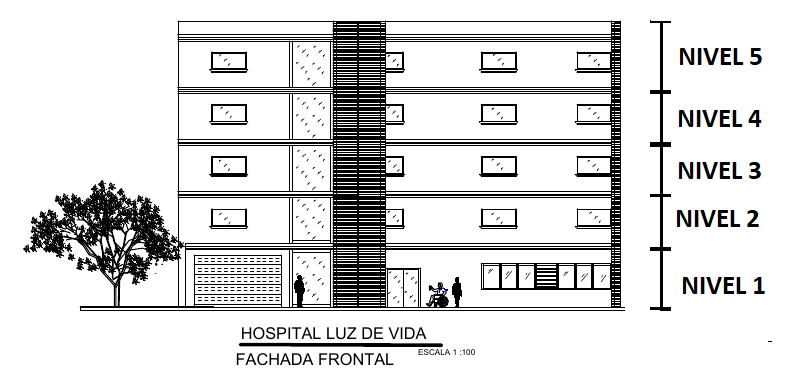
\includegraphics[width=0.9\textwidth]{niveles.png}
	
		\label{fig:mi_imagen}
	\end{figure}
	
	\vspace{0.5cm}
	
	% ===============================
	\subsection{Marco normativo aplicable}
	
	De acuerdo con la \textbf{Norma de Seguridad Estructural de Guatemala NSE-2:2024 – Demandas estructurales y condiciones de sitio}, el período fundamental de vibración de una estructura es un parámetro esencial para:
	
	\begin{itemize}
		\item La selección del espectro sísmico de diseño.
		\item La determinación de las fuerzas sísmicas equivalentes.
		\item La evaluación del comportamiento dinámico global de la edificación.
	\end{itemize}
	
	La norma permite que, en etapas preliminares de diseño, el período fundamental pueda estimarse mediante \textbf{expresiones empíricas}, las cuales proporcionan una aproximación razonable del comportamiento dinámico esperado.
	
	% ===============================
	\subsection{Expresión empírica para el período fundamental}
	
	La \textbf{NSE-2:2024}, manteniendo compatibilidad con la normativa internacional \textbf{ASCE 7-22}, establece que el período fundamental aproximado puede estimarse mediante la expresión:
	
	\begin{equation}
		T_a = C_t \cdot h_n^{\,x}
	\end{equation}
	
	\textbf{Donde:}
	
	\begin{itemize}
		\item $T_a$ = período fundamental empírico de la estructura (s).
		\item $h_n$ = altura total de la edificación medida desde la base hasta el nivel superior (m).
		\item $C_t, x$ = coeficientes empíricos dependientes del sistema estructural.
	\end{itemize}
	
	Esta expresión es válida para \textbf{estructuras regulares} y resulta particularmente útil en la fase de \textbf{anteproyecto}.
	
	% ===============================
	\subsection{Características del Hospital Luz Vida consideradas en el cálculo}
	
	\subsubsection*{Sistema estructural}
	
	El Hospital Luz Vida se proyecta como una edificación de \textbf{concreto reforzado}, organizada mediante \textbf{pórticos resistentes a momento}, sistema compatible con edificaciones hospitalarias y con los criterios de ductilidad exigidos por la normativa sísmica vigente.
	
	De acuerdo con la Tabla~12.8-2 de la normativa ASCE/SEI~7 (Values of Approximate Period Parameters $C_t$ and $x$), los coeficientes empíricos para estructuras de \textbf{PORTICOS RESISTENTES A MOMENTO DE CONCRETO REFORZADO} son:
	
	
		\begin{figure}[H]
		\centering
		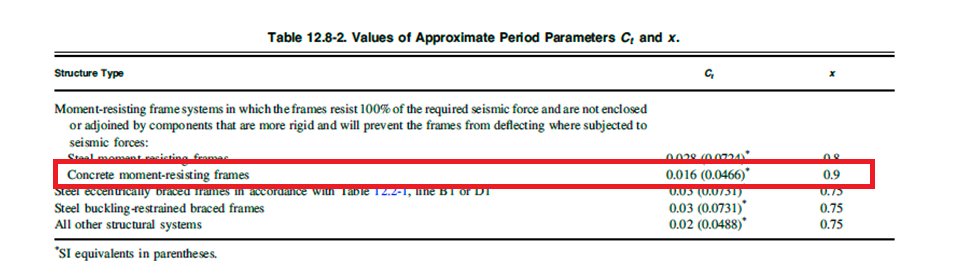
\includegraphics[width=1.2\textwidth]{tabla.png}
		
		\label{fig:mi_imagen}
	\end{figure}
	
	
	
		
	\begin{itemize}
		\item $C_t = 0.0466$
		\item $x = 0.9$
	\end{itemize}
	
	\subsubsection*{Altura total de la edificación}
	
	De acuerdo con el anteproyecto:
	
	\begin{itemize}
		\item Nivel 1: 3.50 m
		\item Niveles 2, 3, 4 y 5: $4 \times 3.00 = 12.00$ m
	\end{itemize}
	
	Por lo tanto:
	
	\begin{equation}
		h_n = 3.50 + 12.00 = 15.50 \ \text{m}
	\end{equation}
	
	% ===============================
	\subsection{Cálculo del período fundamental empírico}
	
	Sustituyendo los valores en la expresión empírica:
	
	\begin{equation}
		T_a = 0.0466 \cdot (15.50)^{0.9}
	\end{equation}
	
	Evaluando la potencia:
	
	\begin{equation}
		(15.50)^{0.9} \approx 11.74
	\end{equation}
	
	Multiplicando:
	
	\begin{equation}
		T_a = 0.0466 \cdot 11.74
	\end{equation}
	
	Por lo tanto:
	
	\begin{equation}
		\boxed{T_a \approx 0.55 \ \text{segundos}}
	\end{equation}
	
	% ===============================

	
	% ===============================
	
	
	\begin{quote}
		De conformidad con la Norma de Seguridad Estructural NSE-2:2024, el período fundamental empírico constituye una aproximación válida del comportamiento dinámico global de la edificación en etapas iniciales del diseño estructural. Para fases posteriores, la normativa establece que dicho período deberá obtenerse a partir de un modelo estructural analítico que represente adecuadamente la masa, rigidez y condiciones de apoyo de la estructura.
	\end{quote}
	
	% ===============================

	
	

	
	

	
	
	
	
	
	
	
	
	
	
	
	
	%%%%%%%%%%%%%%%%%%%%%%%%%%%%%%%%%%%%%%%%%%%%%%%%555
	
		\newpage
	
	% ----------------------------------

	\section{Conclusión}
	Por lo tanto el estudio de los pórticos resistentes a momento permite comprender la importancia de un diseño estructural adecuado frente a acciones sísmicas, donde la ductilidad, la resistencia y la capacidad de disipación de energía juegan un papel determinante en la seguridad de las edificaciones. A lo largo del desarrollo de este trabajo se evidenció que la correcta selección del tipo de pórtico —especial, intermedio u ordinario— depende directamente del nivel de amenaza sísmica, del uso de la edificación y de los requerimientos normativos aplicables. \\
	
	El análisis del comportamiento estructural de los pórticos demuestra que la adecuada distribución de momentos, el control de desplazamientos y la aplicación del diseño por capacidad permiten evitar mecanismos de falla frágil, favoreciendo un comportamiento inelástico controlado durante eventos sísmicos severos. Asimismo, la clasificación de las estructuras de pórticos según su material, configuración geométrica y comportamiento estático facilita una mejor comprensión de su respuesta estructural y de las estrategias de diseño más apropiadas.
	
	% ----------------------------------
	%         BIBLIOGRAFÍA APA
	% ----------------------------------
	\newpage

	
	\bibliographystyle{apacite}
\renewcommand{\refname}{Referencias}

\bibliography{bibliografia}


\renewcommand{\refname}{Referencias}

American Concrete Institute. (2019). \textit{Building code requirements for structural concrete (ACI 318-19) and commentary}. American Concrete Institute.


American Concrete Institute. (2014). \textit{Guide to durable concrete (ACI 201.2R-16)}. American Concrete Institute.





American Concrete Institute. (2014). \textit{Guide to durable concrete (ACI 201.2R-16)}. American Concrete Institute.

Asociación Guatemalteca de Ingeniería Estructural y Sísmica. (2018). \textit{Norma de seguridad estructural NSE 1: Cargas para diseño estructural}. AGIES.

Asociación Guatemalteca de Ingeniería Estructural y Sísmica. (2018). \textit{Norma de seguridad estructural NSE 2: Diseño por sismo}. AGIES.

Asociación Guatemalteca de Ingeniería Estructural y Sísmica. (2018). \textit{Norma de seguridad estructural NSE 3: Concreto estructural}. AGIES.

Asociación Guatemalteca de Ingeniería Estructural y Sísmica. (2018). \textit{Norma de seguridad estructural NSE 4: Acero estructural}. AGIES.

Asociación Guatemalteca de Ingeniería Estructural y Sísmica. (2018). \textit{Norma de seguridad estructural NSE 5: Cimentaciones}. AGIES.

Asociación Guatemalteca de Ingeniería Estructural y Sísmica. (2018). \textit{Normas de seguridad estructural de edificaciones en Guatemala}. AGIES.

Ching, F. D. K. (2015). \textit{Building construction illustrated} (5th ed.). John Wiley \& Sons.

	
	
	
		
	
		
	
	
	
\end{document}